\documentclass[12pt]{article}
\usepackage{graphicx}
\usepackage{amsmath}
\usepackage{mathtools}
\usepackage{gensymb}

\newcommand{\mydet}[1]{\ensuremath{\begin{vmatrix}#1\end{vmatrix}}}
\providecommand{\brak}[1]{\ensuremath{\left(#1\right)}}
\providecommand{\norm}[1]{\left\lVert#1\right\rVert}
\newcommand{\solution}{\noindent \textbf{Solution: }}
\newcommand{\myvec}[1]{\ensuremath{\begin{pmatrix}#1\end{pmatrix}}}
\let\vec\mathbf

\begin{document}
\begin{center}
\textbf\large{CHAPTER-7 \\ TRIANGLES}
\end{center}
\section*{Excercise 7.1}

Q1. Which of the following is not a criterion for congruence of triangles$?$
\begin{enumerate}
\item $SAS$
\item $ASA$
\item $SSA$
\item $SSS$
\end{enumerate}

\solution
\begin{enumerate}
\item $SAS(Side-Angle-Side)$ rule is used to prove the congruency of triangles.\\
It states that , if two sides and the included angle of one triangle are equal to two sides and included angle of another triangle,then the triangles are said to be in congruent.An included angles is an angle formed by two given sides.\\
		For triangles $PQR$ and $XYZ$, if $PQ = XZ$, $PR = YZ$ and $\angle Z <= \angle P$ , then by $SAS$ rule , $\triangle XYZ \text{ is } \cong \text{ to }  \triangle PQR$  as shown in Figure\ref{fig:Fig2}.
		\begin{figure}[!h]
  \begin{center} 
      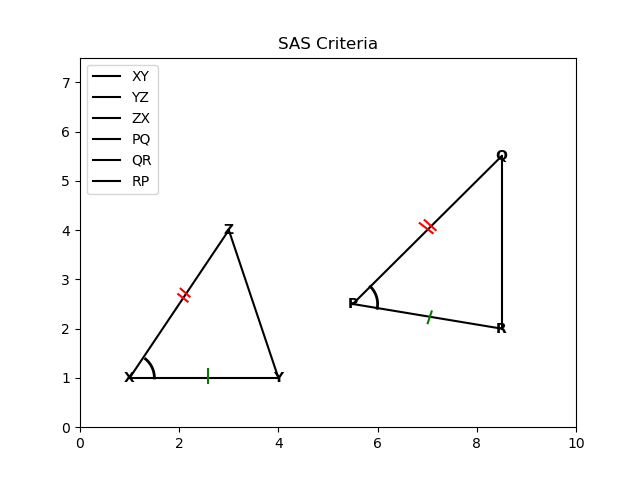
\includegraphics[width=\columnwidth]{./figs/graph2.png}
  \end{center}
\caption{}
\label{fig:Fig2}
\end{figure}
\pagebreak
\item $ASA(Angle-Side-Angle)$ rule is used to prove the congruency of triangles.\\
It states that , if two angles and a non-included side of one triangle are equal to two angles and a non-included side of another triangle,then the triangles are said to be in congruent.\\
		For triangles $PQR$ and $XYZ$ ,$XZ = QP$ , $ \angle X = \angle Q$ , and $\angle Y = \angle R$ , then $\triangle XYZ \text{ is } \cong \text{ to }  \triangle PQR$ as shown in Figure\ref{fig:Fig1}.
		\begin{figure}[!h]
  \begin{center} 
      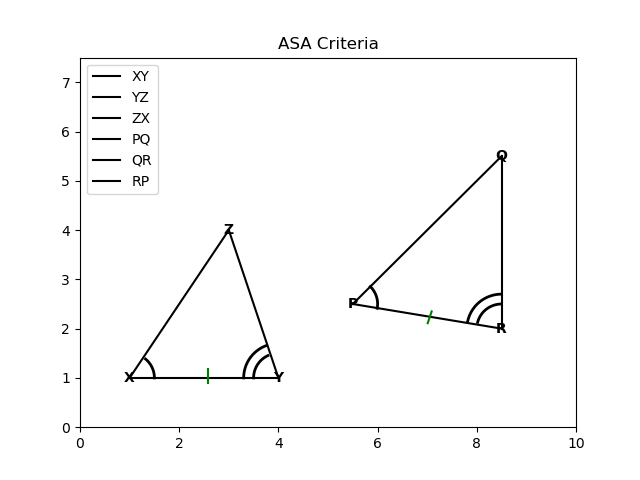
\includegraphics[width=\columnwidth]{./figs/graph1.png}
  \end{center}
\caption{}
\label{fig:Fig1}
\end{figure}
\pagebreak
\item $SSA$ there is no such criterion postulated.
\item $SSS(Side-Side-Side)$ rule is also used to prove the congruency of triangles.\\
	If three sides of one triangle are equal to three sides of another triangle , then the triangles are congruent.\\
For triangles $PQR$ and $XYZ$ , if $XY = PR$ , $YZ = PQ$ and $ZX = QR$ , then $\triangle XYZ \text{ is } \cong \text{ to }  \triangle PQR$ as shown in Figure:\ref{fig:Fig3}.
\begin{figure}[!h]
  \begin{center} 
      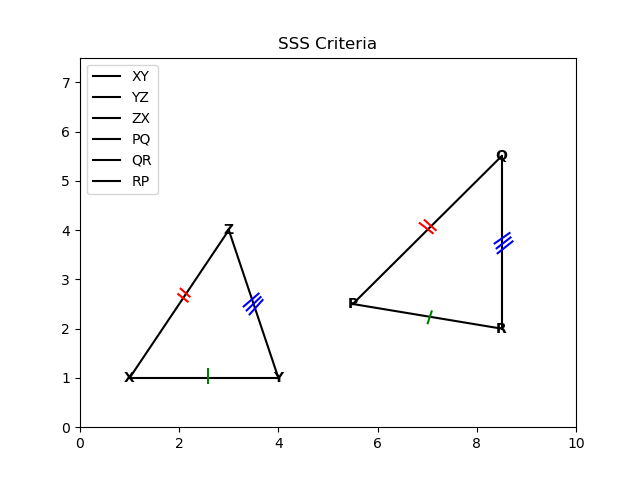
\includegraphics[width=\columnwidth]{./figs/graph3.png}
  \end{center}
\caption{}
\label{fig:Fig3}
\end{figure}
\end{enumerate}
\end{document}
